\begin{frame}
\frametitle{Pilot Logbooks}
\begin{block}{CASR1998 REG 61.345 \emph{(pilot logbooks)}}
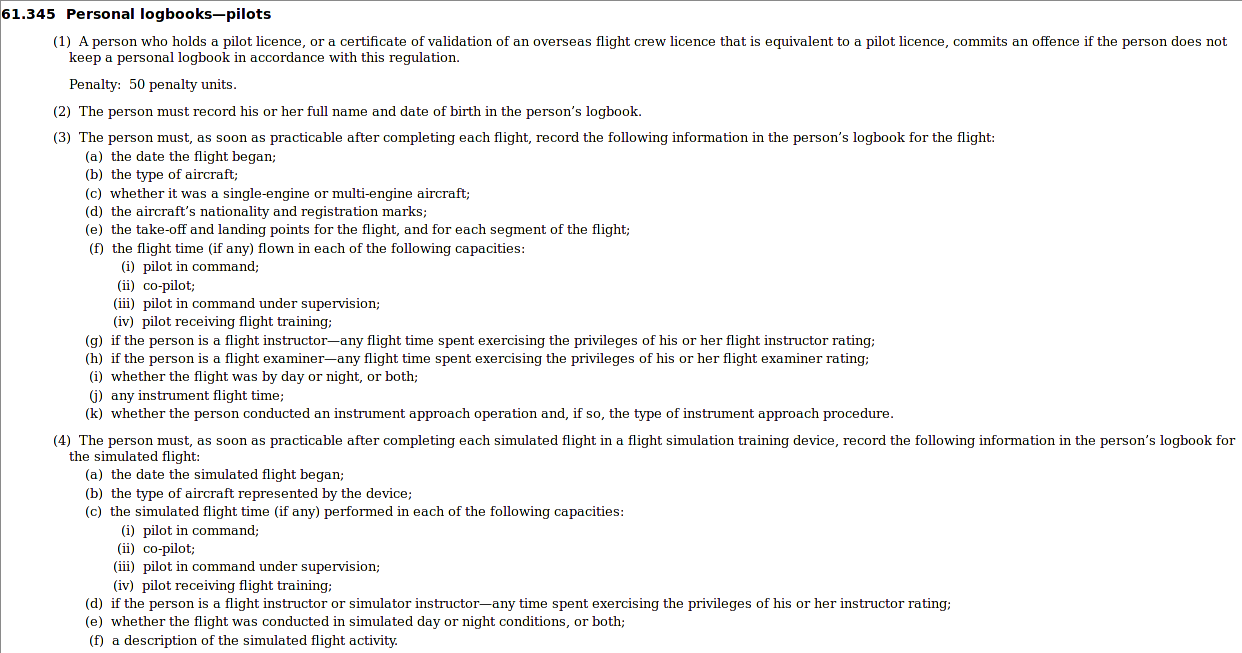
\includegraphics[height=0.6\textheight]{image/casr-logbook.png}
\end{block}
\end{frame}

\begin{frame}
\frametitle{Pilot Logbooks}
\begin{block}{Here is a typical pilot logbook}
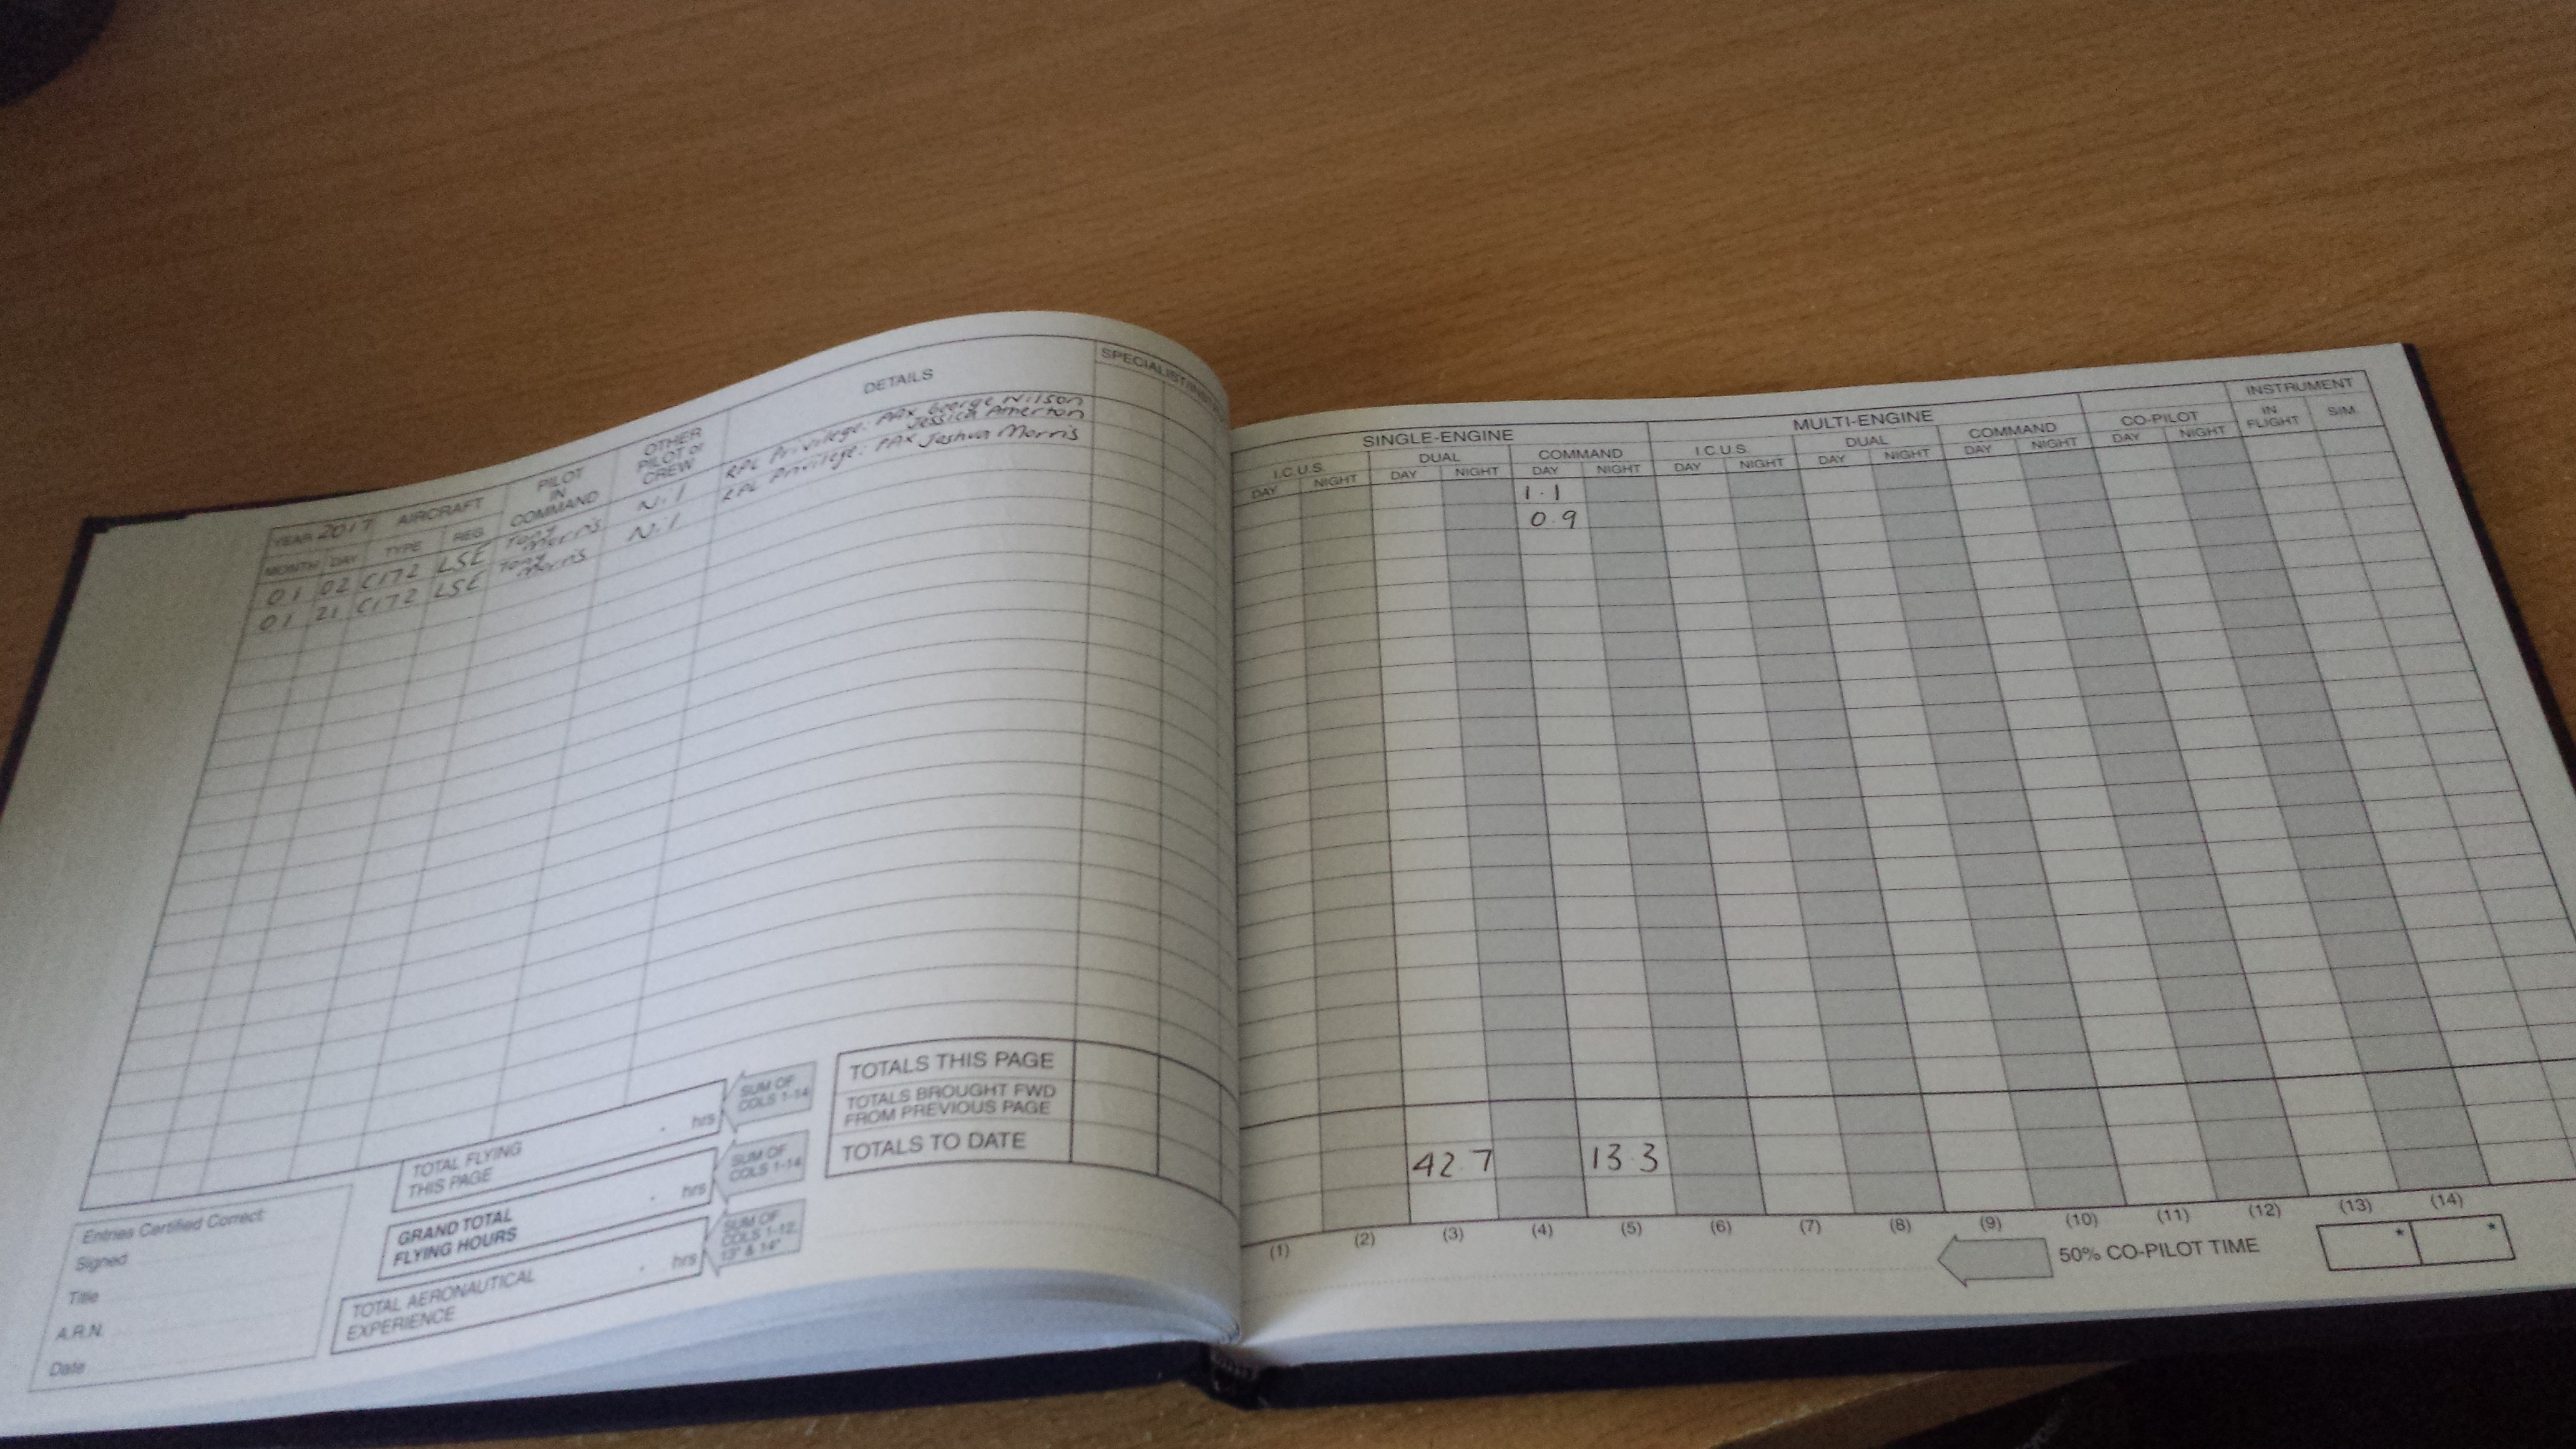
\includegraphics[height=0.5\textheight]{image/logbook.jpg}
\end{block}
\end{frame}

\begin{frame}
\frametitle{Pilot Logbooks}
\begin{block}{CASR1998 REG 61.345 \emph{(pilot logbooks)}}
Are electronic logbooks OK?
\end{block}
\end{frame}

\begin{frame}
\frametitle{Pilot Logbooks}
\begin{block}{Yes. CASR1998 REG 61.365(3)}
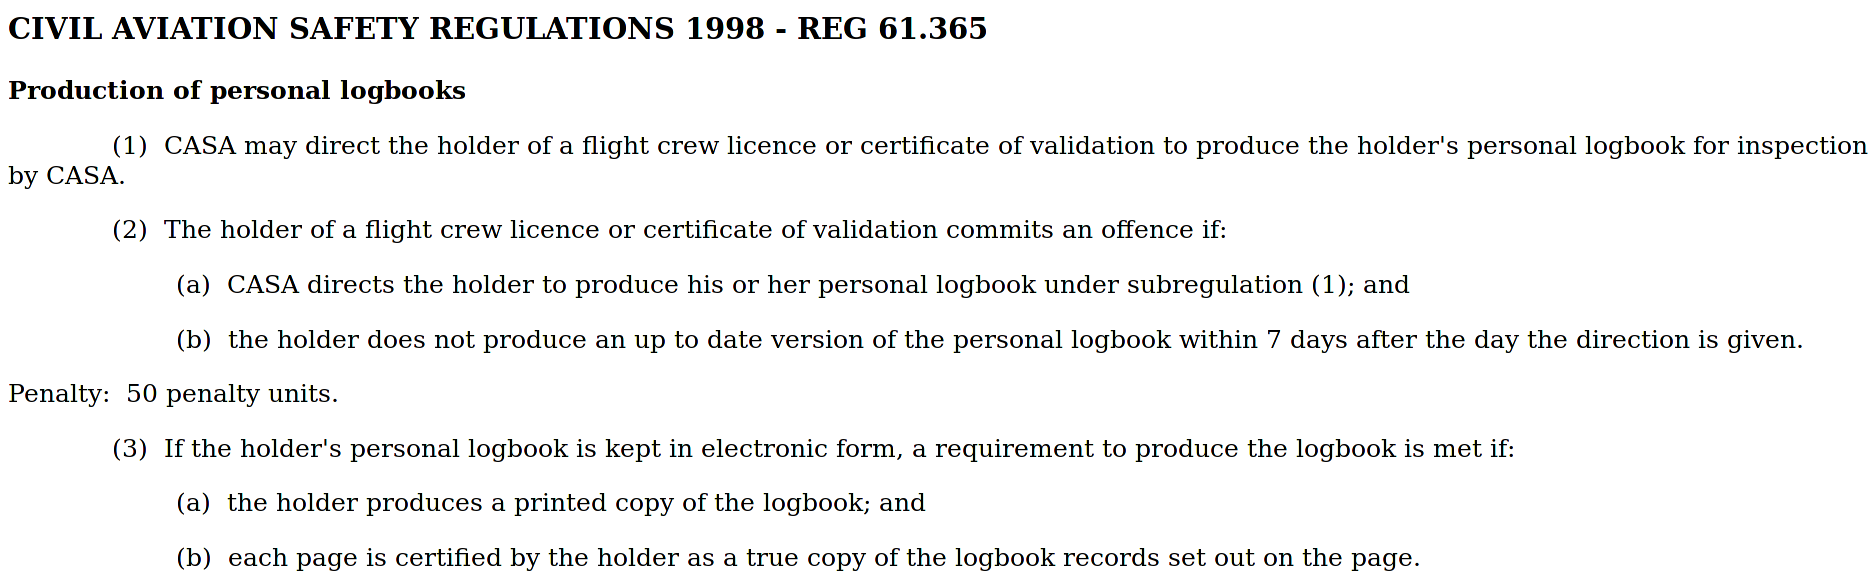
\includegraphics[height=0.3\textheight]{image/casr-logbook-production.png}
\end{block}
\end{frame}

\begin{frame}
\frametitle{Pilot logbooks}
\begin{center}
Introducing the pilot logbook cottage industry
\par

\includegraphics[height=0.1\textheight]{image/reddit-logbooks.png}
\end{center}
\end{frame}

\begin{frame}
\frametitle{Introducing the pilot logbook cottage industry}
\begin{block}{Excel?}

\includegraphics[height=0.1\textheight]{image/logbook-1.png}
\end{block}
\end{frame}

\begin{frame}
\frametitle{Introducing the pilot logbook cottage industry}
\begin{block}{Google spreadsheet?}
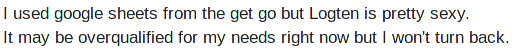
\includegraphics[height=0.1\textheight]{image/logbook-2.png}
\end{block}
\end{frame}

\begin{frame}
\frametitle{Introducing the pilot logbook cottage industry}
\begin{block}{proprietary logbook software?}
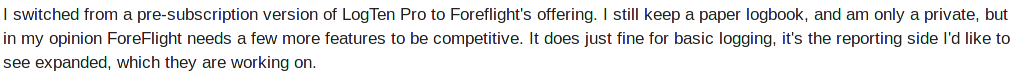
\includegraphics[height=0.08\textheight]{image/logbook-3.png}
\end{block}
\end{frame}

\begin{frame}
\frametitle{Introducing the pilot logbook cottage industry}
\begin{block}{I love proprietary software!}

\includegraphics[height=0.05\textheight]{image/logbook-4.png}
\end{block}
\end{frame}

\begin{frame}
\frametitle{Introducing the pilot logbook cottage industry}
\begin{block}{I hate proprietary software when it doesn't work}

\includegraphics[height=0.05\textheight]{image/logbook-5.png}
\end{block}
\end{frame}

\begin{frame}
\frametitle{Introducing the pilot logbook cottage industry}
\begin{block}{I hate proprietary software when I cross the date line}

\includegraphics[height=0.05\textheight]{image/logbook-6.png}
\end{block}
\end{frame}

\begin{frame}
\frametitle{Introducing the pilot logbook cottage industry}
\begin{block}{umm where's my logbook gone?}
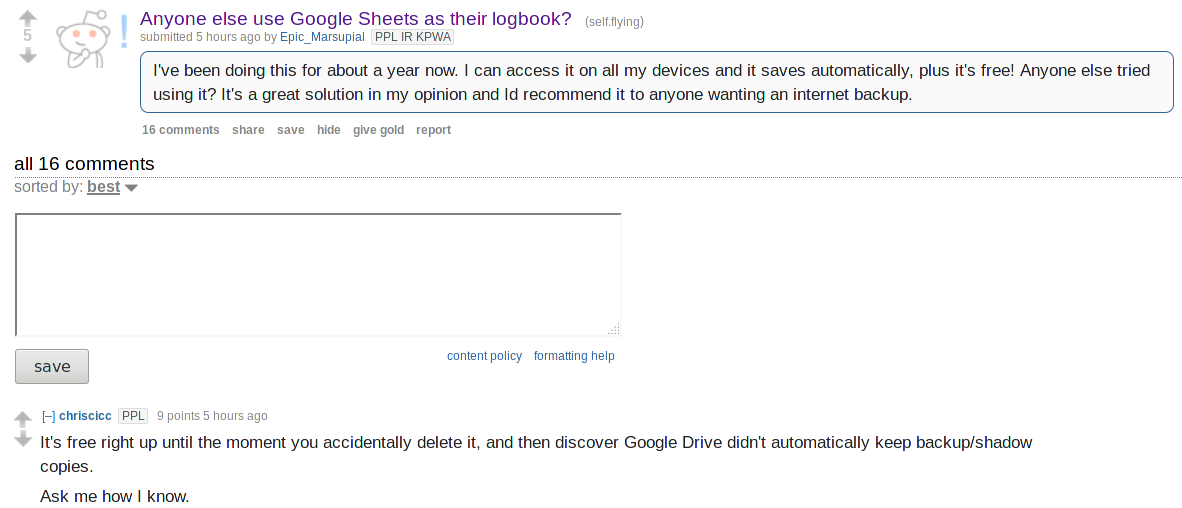
\includegraphics[height=0.4\textheight]{image/logbook-7.png}
\end{block}
\par
\tiny{\emph{01 August 2016}}
\end{frame}

\begin{frame}
\frametitle{Pilot logbook}
\begin{block}{A responsible, CASR1998 REG 61.x compliant pilot uses}
\begin{itemize}
\item<1-> Haskell data type (sums and products) for logbook.
\item<1-> Lenses, Prisms and Traversals for querying and reporting.
\item<1-> Pilot logbook zipper for navigating a logbook.
\item<1-> A pretty-printer to meet CASR1998 REG 61.365 requirements.
\item<1-> Revision control (git) for mitigating data loss.
\item<1-> Publishes open-source logbook libraries as a good citizen.
\end{itemize}
\end{block}
\end{frame}

\begin{frame}
\frametitle{Pilot logbook}
\begin{block}{lenses? zippers?}
\begin{itemize}
\item<1-> what is a lens?
\item<1-> prism?
\item<1-> zipper?
\item<1-> WHAT?
\end{itemize}
\end{block}
\end{frame}

\begin{frame}
\frametitle{Pilot logbook}
\begin{block}{Here is the problem}
\begin{itemize}
\item<1-> We all know and agree that immutable objects have significant advantages for our code.
\item<1-> This idea has been known since the 1930s as: Functional Programming.
\end{itemize}
\end{block}
\end{frame}

\begin{frame}
\frametitle{Pilot logbook}
\begin{block}{Here is the problem}
\begin{itemize}
\item<1-> but a na{\"\i}ve effort toward achieving this thesis results in several, significant practical problems.
\item<1-> and we are somewhat aware of these problems.
\end{itemize}
\end{block}
\end{frame}

\begin{frame}
\frametitle{Pilot logbook}
\begin{block}{For example}
given a logbook\ldots
\begin{itemize}
\item that has an aviator\ldots
\item that has an ARN\ldots
\item that has 0 or many digits\ldots
\end{itemize}
find the first digit that is even and, if it exists, add 1 to it
\end{block}
\emph{Logbook.java}
\end{frame}

% Here is the problem
% We all know and agree that immutable objects have significant advantages for our code. We generally call this idea: Functional Programming.
% but a na{\"\i}ve effort toward achieving this thesis results in several, significant practical problems

% For example, given a logbook, that has an aviator, that has an ARN, that has 0 or many digits...
% find the first digit that is even and, if it exists, then add 1 to it.

\begin{frame}[fragile]
\frametitle{Use-case}
\begin{block}{Modify: Find the first digit that is even and, if it exists, add 1 to it}
\begin{lstlisting}[style=haskell,basicstyle=\scriptsize\ttfamily,mathescape]
$\lambda$> :t over (singular
        ( 
          logbook .
          logbookaviator .
          arn .
          traverse .
          filtered digiteven
        )
      )
      successor
Logbook -> Logbook
\end{lstlisting}
\end{block}
\end{frame}

\begin{frame}[fragile]
\frametitle{Use-case}
\begin{block}{Query: Aircraft from all flights}
% logbookentries :: Lens Logbook Entries
% _Wrapped :: Iso$'$ Entries [Entry]
% folded :: Foldable f => IndexedFold Int (f a) a 
% _AircraftFlightEntry ::
%       Prism$'$ Entry AircraftFlight
% flightaircraft :: Lens$'$ AircraftFlight Aircraft
% mylogbook :: Logbook
\begin{lstlisting}[style=haskell,basicstyle=\scriptsize\ttfamily,mathescape]
$\lambda$> :t mylogbook ^..
      logbook .
      logbookentries .
      _Wrapped .
      folded .
      _AircraftFlightEntry .
      flightaircraft
[Aircraft]
\end{lstlisting}
\end{block}
\end{frame}

\begin{frame}[fragile]
\frametitle{Use-case}
\begin{block}{Query: Find first flight in aircraft registration VH-VVO}
% logbookentries :: Lens Logbook Entries
% _AircraftFlightEntry ::
%       Prism$'$ Entry AircraftFlight
% flightaircraft :: Lens$'$ AircraftFlight Aircraft
% aircraftRegistration :: Lens$'$ Aircraft String
\begin{lstlisting}[style=haskell,basicstyle=\scriptsize\ttfamily,mathescape]
$\lambda$> :t findOf
      ( logbook . 
        logbookentries . 
        _Wrapped . 
        folded . 
        _AircraftFlightEntry)
        ( elemOf
          (
            flightaircraft . 
            aircraftRegistration)
          "VH-VVO")
      mylogbook
Maybe AircraftFlight
\end{lstlisting}
\end{block}
\end{frame}

\begin{frame}[fragile]
\frametitle{Use-case}
\begin{block}{Query: Total day hours as pilot in-command}
\begin{lstlisting}[style=haskell,basicstyle=\scriptsize\ttfamily,mathescape]
$\lambda$> foldOf
      ( logbook .
        logbookentries .
        _Wrapped .
        folded .
        _AircraftFlightEntry .
        filtered
          (elemOf (command . _InCommand) ()) .
        daynight .
        dayDayNight
      )
      mylogbook
TimeAmount {_hours = 4, _tenthofhour = 8}
\end{lstlisting}
\end{block}
\end{frame}

\begin{frame}[fragile]
\frametitle{Use-case}
\begin{block}{Print the entire logbook to a single, printable HTML web page \emph{CASR1998 REG 61.365}}
\begin{lstlisting}[style=haskell,mathescape]
$\lambda$> :t htmlLogbook mylogbook
Html ()
\end{lstlisting}
\end{block}
\href{http://logbook.aviation.tmorris.net/}{http://logbook.aviation.tmorris.net/}
\end{frame}

\begin{frame}[fragile]
\frametitle{Use-case}
\begin{block}{Query of arbitrary obtuseness}
All flights where, if the departure and arrival date is the same day (UTC), and that date-of-month is a multiple of 7, unless either there was an intermediate flight path point of YSCN, or the time the logbook owner was PiC for the first three legs of the flight, is between 2.0 hours and the total sum of hours of dual flight in aircraft registered VH-AFR.
\end{block}
\end{frame}

\begin{frame}[fragile]
\frametitle{Use-case}
\begin{block}{What is the goal?}
\begin{itemize}
\item<1-> The effort required to perform a query or update is directly proportional to the sophistication of that operation.
\item<2-> Counting, querying, searching, updating, filtering, tabulating, transposing, intercalating, grouping, partitioning, indexing, unioning, intersecting on data in a pilot logbook is not only physically laborious, but prone to error.
\item<3-> Yet this procedure is executed manually every day at airports.
\end{itemize}

\end{block}
\end{frame}

\begin{frame}[fragile]
\frametitle{Use-case}
\begin{block}{}
\begin{itemize}
\item<1-> In training, pilots are examined on, and seem to enjoy, doing the computer's job so it doesn't have to.
\item<2-> I call this \emph{Flesh Computing}.
\end{itemize}
\end{block}
\end{frame}
